\chapter{Cơ sở lý thuyết và các nghiên cứu liên quan}
\label{ch:co-so-ly-thuyet}

Chương này trình bày cơ sở lý thuyết y sinh học và phương pháp luận học máy nền tảng cho bài toán dự đoán mức độ triệu chứng trầm cảm từ dữ liệu sinh lý dạng bảng, đồng thời điểm qua các công trình nghiên cứu tiền nhiệm. Nội dung chương gồm: (1) Cấu trúc thang đo PHQ-9 và các cơ chế sinh học liên quan; (2) Hai đặc thù của dữ liệu y tế dạng bảng gồm mất cân bằng lớp và chồng lấn phân phối đặc trưng; (3) Khảo sát các thuật toán cơ sở và đi sâu vào thuật toán Random Forest; (4) Ba trường phái mô hình hóa gồm phân loại phẳng, phân loại phân cấp kết hợp lý thuyết quyết định nhạy chi phí Bayes, và phân loại thứ bậc; (5) Tổng hợp các nghiên cứu liên quan.

\section{Thang đo PHQ-9 và cơ sở sinh lý học của triệu chứng trầm cảm}
\label{sec:thang-do-phq9-va-sinh-ly}

\subsection{Cấu trúc thang đo PHQ-9 và phân khoảng mức độ}
\label{subsec:cau-truc-phq9}

Thang đo Sức khỏe Bệnh nhân 9 mục (Patient Health Questionnaire-9 -- PHQ-9) là công cụ sàng lọc tâm thần tự báo cáo được chuẩn hóa, do Kroenke, Spitzer và Williams phát triển \cite{kroenke2001phq, spitzer1999validation}. PHQ-9 gồm 9 câu hỏi phản ánh tần suất xuất hiện các biểu hiện trong vòng hai tuần gần nhất, tương ứng với tiêu chuẩn DSM-IV: (1) Giảm hứng thú hoặc niềm vui trong các hoạt động; (2) Cảm giác buồn bã, chán nản hoặc tuyệt vọng; (3) Rối loạn giấc ngủ; (4) Mệt mỏi, thiếu năng lượng; (5) Thay đổi cảm giác thèm ăn; (6) Cảm giác tự ti hoặc mặc cảm tội lỗi; (7) Giảm khả năng tập trung; (8) Vận động chậm chạp hoặc bồn chồn; (9) Ý nghĩ về cái chết hoặc tự làm hại bản thân.

Mỗi câu hỏi được chấm điểm theo thang Likert 4 mức độ từ 0 đến 3 (0: Hoàn toàn không; 1: Vài ngày; 2: Hơn một nửa số ngày; 3: Gần như mỗi ngày). Tổng điểm số $s = \sum_{j=1}^9 \text{DPQ}_j \in [0, 27]$ được ánh xạ thành 5 khoảng mức độ triệu chứng được minh họa trong Hình \ref{fig:phq9-tiers}.

\begin{figure}[htbp]{Thang đo PHQ-9 (0--27 điểm), 5 khoảng mức độ triệu chứng và ánh xạ sang không gian 3 nhóm $T_3$}
\centering
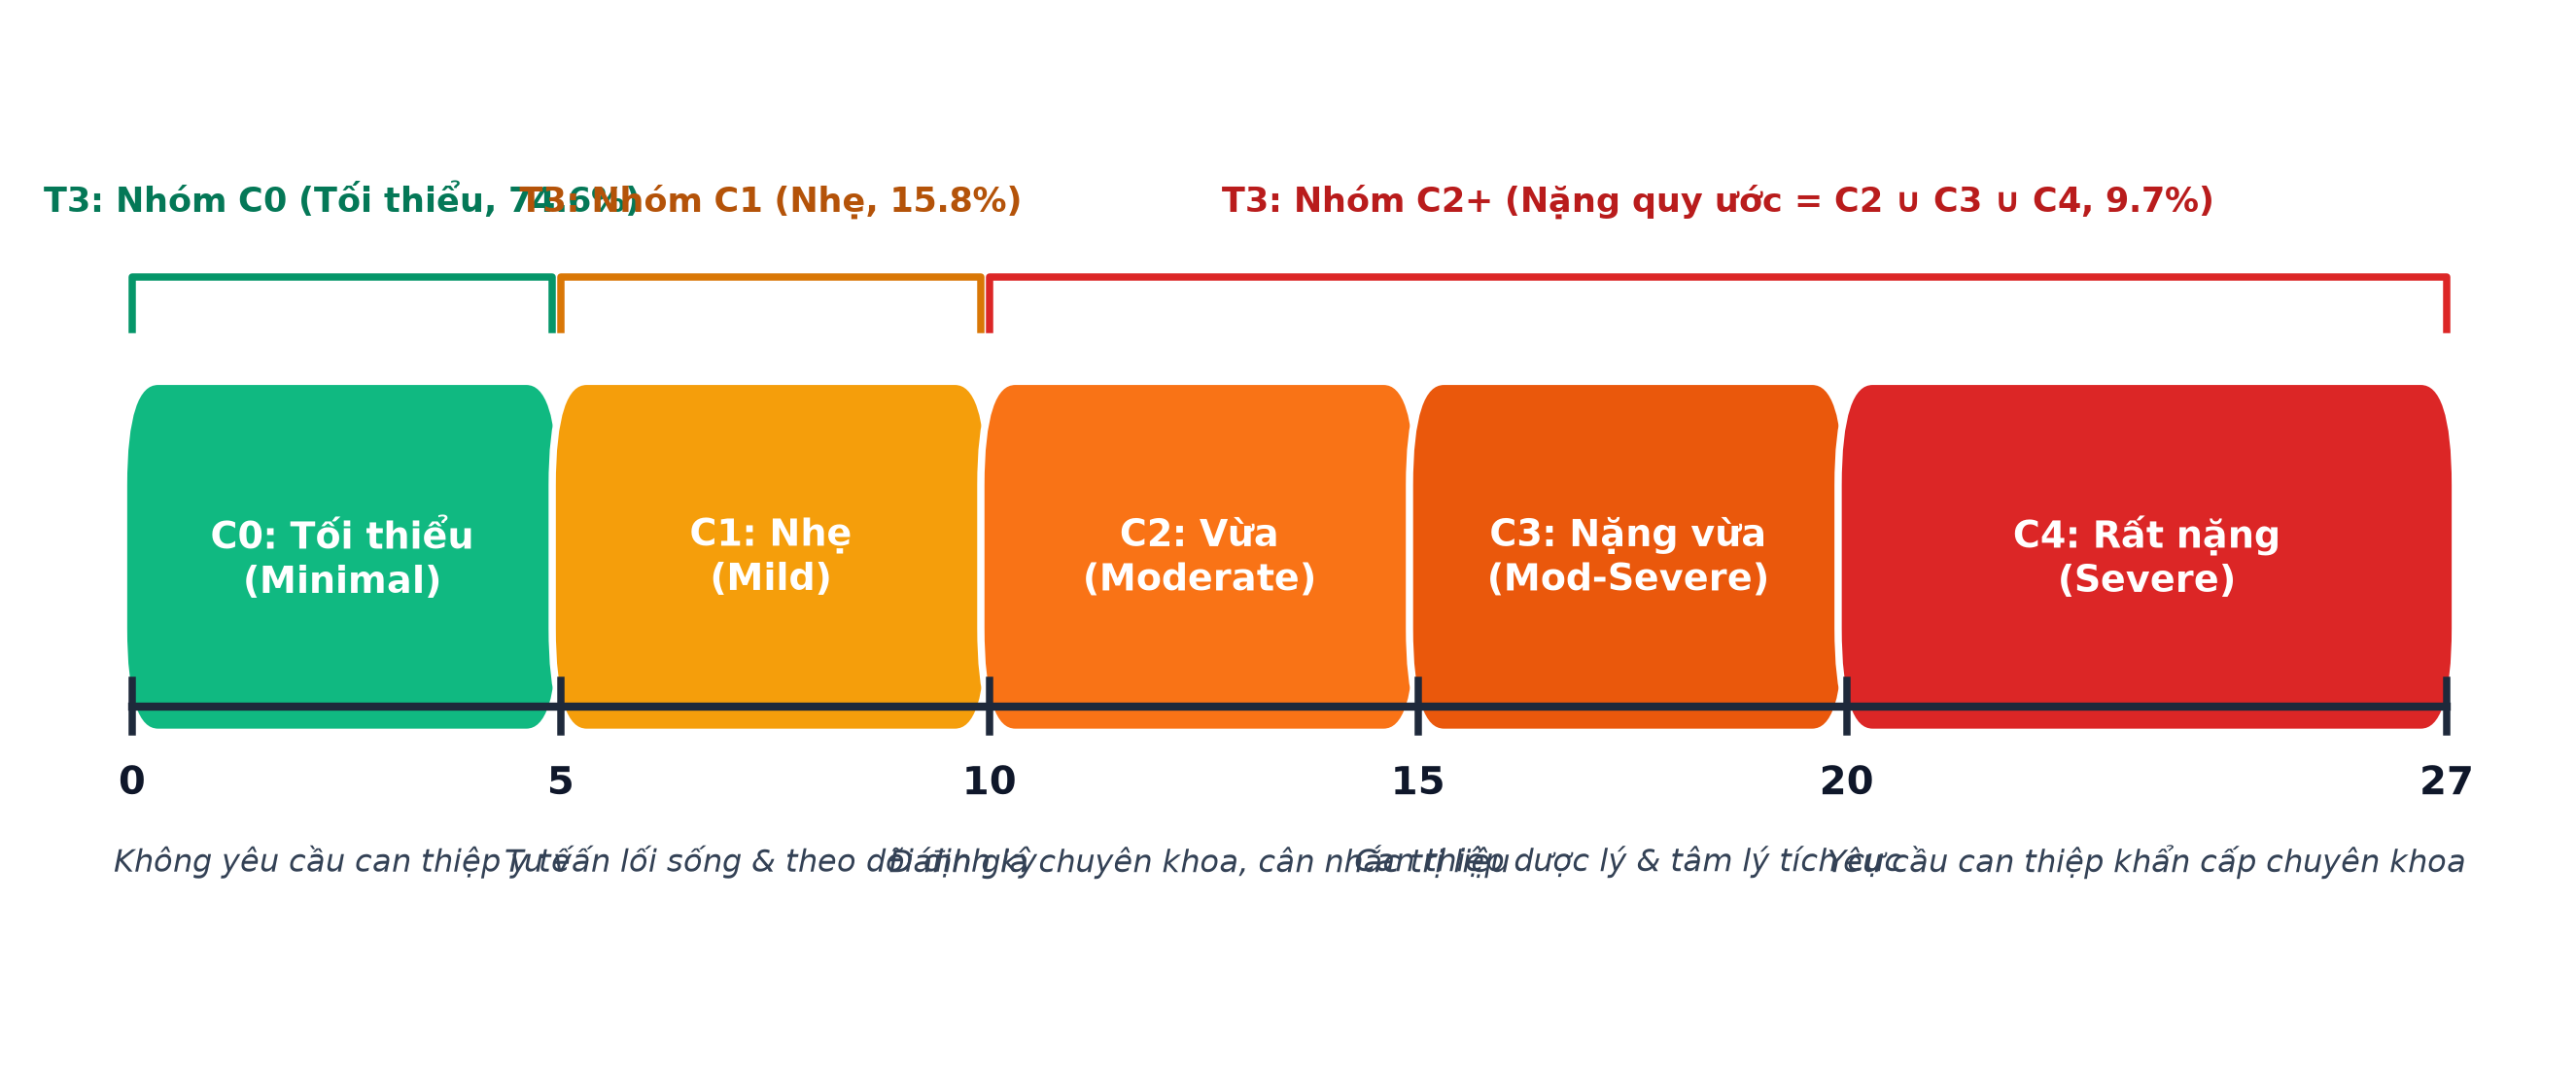
\includegraphics[width=\textwidth]{figures/fig2_phq9_tiers.png}
\label{fig:phq9-tiers}
\end{figure}
\FloatBarrier

Theo quy ước trong y văn:
\begin{itemize}
    \item $s \in [0, 4]$ ($C_0$ -- Tối thiểu): Mức triệu chứng tối thiểu, thường phản ánh trạng thái tâm lý ổn định theo thang đo tự điền.
    \item $s \in [5, 9]$ ($C_1$ -- Nhẹ): Mức độ triệu chứng nhẹ; trong sàng lọc cộng đồng thường được lưu ý theo dõi thêm.
    \item $s \in [10, 14]$ ($C_2$ -- Vừa): Mức độ triệu chứng trung bình; thường được xem là ngưỡng điểm gợi ý cần thăm khám chuyên sâu.
    \item $s \in [15, 19]$ ($C_3$ -- Nặng vừa): Mức độ triệu chứng nặng vừa theo thang đo PHQ-9.
    \item $s \in [20, 27]$ ($C_4$ -- Nặng): Mức độ triệu chứng nặng nhất theo thang đo PHQ-9.
\end{itemize}

Trong đề tài DepSev-ML, bên cạnh không gian 5 mức ban đầu ($T_5$), bài toán còn được khảo sát trên không gian 3 nhóm ($T_3$), trong đó nhóm $C_2^+$ đại diện cho toàn bộ các mẫu có điểm PHQ-9 $\ge 10$ ($C_2 \cup C_3 \cup C_4$), được gọi là nhóm Nặng theo quy ước nghiên cứu. Cần lưu ý rằng các khoảng điểm này đóng vai trò nhãn mục tiêu cho bài toán học máy, không đồng nghĩa với chẩn đoán xác định bệnh học lâm sàng.

\subsection{Cơ sở sinh lý học và các chỉ số liên quan}
\label{subsec:co-so-sinh-ly}

Dù triệu chứng trầm cảm thể hiện chủ yếu qua cảm xúc và hành vi, các nghiên cứu y sinh học ghi nhận mối liên hệ giữa trạng thái trầm cảm và một số rối loạn chuyển hóa, miễn dịch ngoại vi thông qua trục não-ruột và trục hạ đồi-tuyến yên-tuyến thượng thận (HPA) \cite{pratt2014depression}.

\begin{figure}[htbp]{Các cơ chế y sinh học liên kết chỉ số sinh lý ngoại vi với mức độ triệu chứng trầm cảm}
\centering
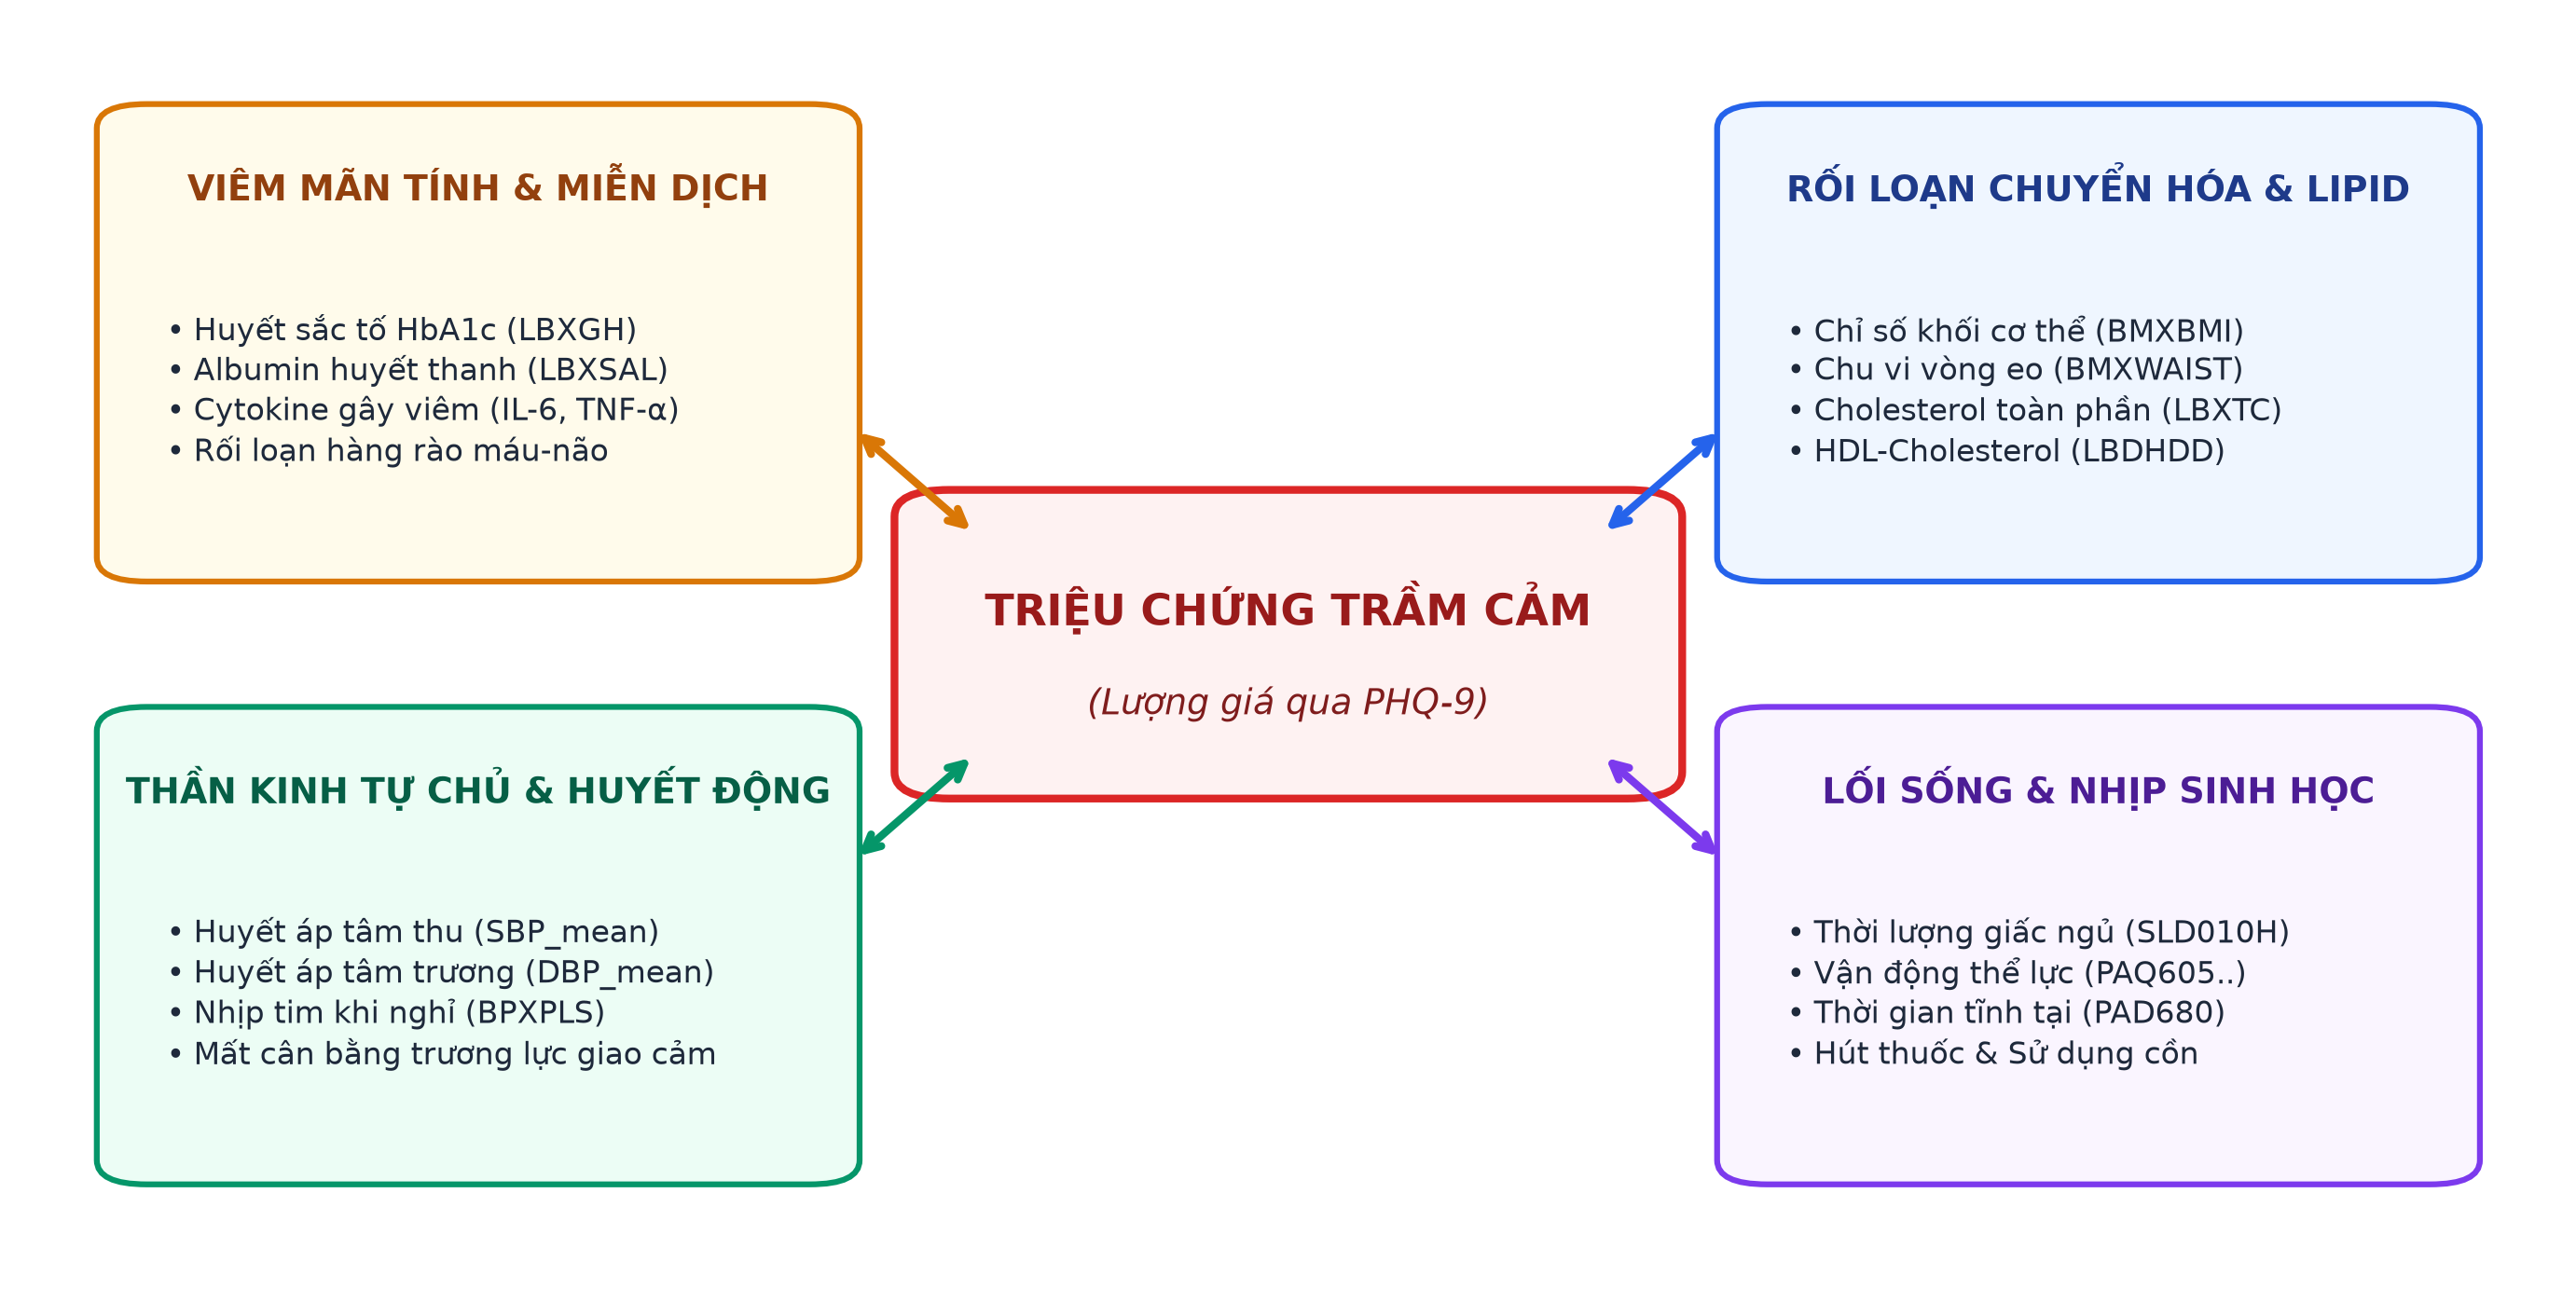
\includegraphics[width=\textwidth]{figures/fig2_gut_brain_metabolic_axis.png}
\label{fig:gut-brain-axis}
\end{figure}
\FloatBarrier

Như mô tả trong Hình \ref{fig:gut-brain-axis}, các nhóm biến số ngoại vi trong NHANES liên quan đến bốn cơ chế chính:
\begin{enumerate}
    \item \textbf{Phản ứng viêm và miễn dịch ngoại vi:} Trầm cảm có thể liên quan đến các cytokine gây viêm ngoại vi. Nồng độ Albumin huyết thanh (LBXSAL) phản ánh tình trạng dinh dưỡng và protein huyết tương; chỉ số đường huyết tích lũy Glycohemoglobin HbA1c (LBXGH) phản ánh mức độ chuyển hóa glucose.
    \item \textbf{Chuyển hóa và lipid máu:} Hoạt động chuyển hóa thể hiện qua các chỉ số nhân trắc học như chỉ số khối cơ thể (BMXBMI), chu vi vòng eo (BMXWAIST), kết hợp cùng nồng độ Cholesterol toàn phần (LBXTC) và HDL-Cholesterol (LBDHDD).
    \item \textbf{Hệ thần kinh tự chủ và huyết áp:} Sự thay đổi trương lực giao cảm có thể ảnh hưởng đến nhịp tim khi nghỉ (BPXPLS), huyết áp tâm thu (SBP\_mean) và huyết áp tâm trương (DBP\_mean).
    \item \textbf{Hành vi lối sống:} Thời gian ngủ (SLD010H), mức độ hoạt động thể lực, thời gian ngồi tĩnh tại (PAD680) cùng với hành vi hút thuốc, uống rượu bia có mối tương quan đáng kể với sự gia tăng điểm số PHQ-9.
\end{enumerate}

\section{Đặc thù và thách thức của dữ liệu y tế dạng bảng}
\label{sec:dac-thu-du-lieu-bang}

Dữ liệu y tế dạng bảng trích xuất từ các khảo sát cộng đồng như NHANES có những đặc thù hình học phức tạp, khác biệt căn bản so với dữ liệu hình ảnh hay văn bản.

\subsection{Mất cân bằng lớp (Severe Class Imbalance)}
\label{subsec:mat-can-bang-lop}

Trong các cuộc điều tra dịch tễ học dân số, phần lớn người tham gia thuộc nhóm triệu chứng tối thiểu, trong khi nhóm có triệu chứng nặng chỉ chiếm tỷ lệ nhỏ. Tỷ số mất cân bằng (Imbalance Ratio -- IR) được tính bởi:
\begin{equation}
    \text{IR} = \frac{\max_k N_k}{\min_k N_k}
\end{equation}
Trong tập phát triển Legacy của nghiên cứu ($N = 4.045$), lớp $C_0$ chiếm $3.016$ đối tượng (74.56\%), trong khi lớp nặng nhất $C_4$ chỉ có $44$ đối tượng (1.09\%), tạo nên tỷ số mất cân bằng $\text{IR} = 3016 / 44 \approx 68.5:1$ (Hình \ref{fig:imbalance-overlap}a).

Nếu mô hình học máy huấn luyện nhằm tối thiểu hóa sai số toàn cục thông thường, thuật toán sẽ bị thiên lệch mạnh về phía lớp $C_0$, dẫn tới hiện tượng đạt độ chính xác Accuracy cao nhưng bỏ sót các ca có triệu chứng thực tế. Để giảm thiểu ảnh hưởng này, kỹ thuật gán trọng số nghịch đảo tần số lớp (Class-weighted objective) được áp dụng:
\begin{equation}
    w_k = \frac{N}{K \cdot N_k}
\end{equation}
nhằm cân bằng lại mức độ đóng góp của từng lớp trong quá trình tối ưu hàm mục tiêu.

\begin{figure}[htbp]{(a) Mất cân bằng lớp trên tập dữ liệu và (b) Hiện tượng chồng lấn phân phối đặc trưng sinh lý}
\centering
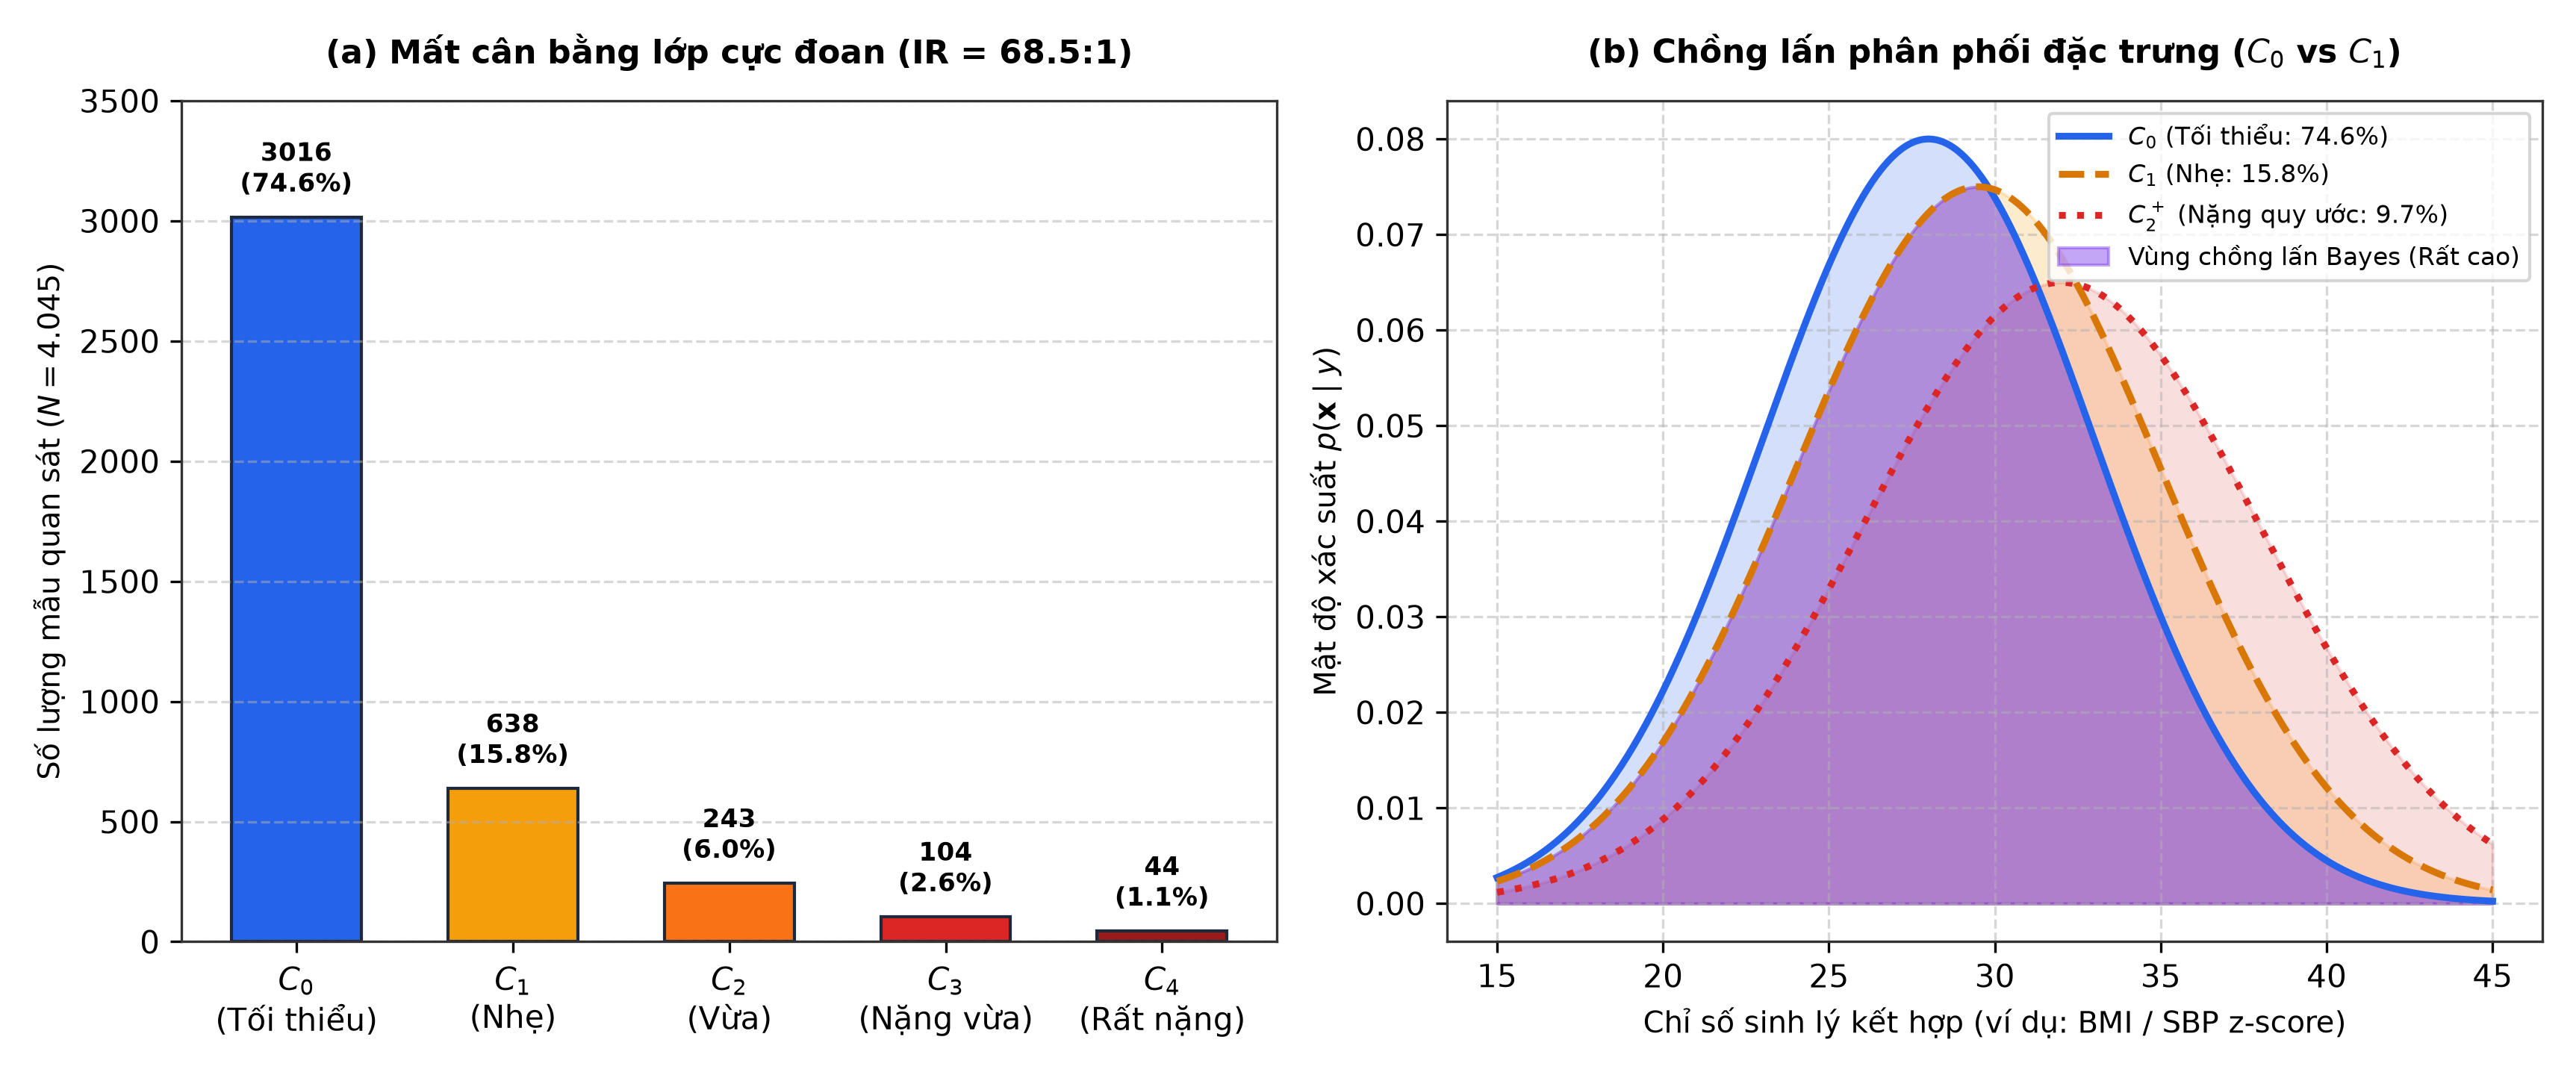
\includegraphics[width=\textwidth]{figures/fig2_imbalance_overlap.png}
\label{fig:imbalance-overlap}
\end{figure}
\FloatBarrier

\subsection{Chồng lấn phân phối đặc trưng (Feature Overlap)}
\label{subsec:chong-lan-dac-trung}

Khác với các xét nghiệm chẩn đoán đặc hiệu, các chỉ số sinh lý như huyết áp, cholesterol hay BMI không có một ngưỡng cắt sinh học duy nhất để phân tách rạch ròi người có triệu chứng tối thiểu và người có triệu chứng nhẹ. Phân phối xác suất điều kiện của đặc trưng $\mathbf{x}$ giữa hai trạng thái kế cận $p(\mathbf{x} \mid Y = 0)$ và $p(\mathbf{x} \mid Y = 1)$ có diện tích giao thoa rất lớn (Hình \ref{fig:imbalance-overlap}b).

Khi vùng giao thoa phân phối sinh lý giữa các lớp lớn, bộ phân loại không thể đạt được độ chính xác phân tách tuyệt đối nếu chỉ dựa vào các biến số sinh lý ngoại vi. Do đó, việc cải thiện hiệu năng đòi hỏi phải lựa chọn cấu trúc bài toán phù hợp và kiểm soát sự đánh đổi giữa các loại sai số.

\section{Khảo sát các thuật toán học máy cơ sở và Thuật toán Random Forest}
\label{sec:cac-thuat-toan-va-rf}

\subsection{Giới thiệu ngắn gọn các thuật toán học máy cơ sở}
\label{subsec:khao-sat-thuat-toan-co-so}

Để xây dựng và đánh giá các mô hình cơ sở (baselines), nghiên cứu đã thử nghiệm 4 thuật toán học máy phổ biến gồm Logistic Regression, Decision Tree, Random Forest và XGBoost:
\begin{itemize}
    \item \textbf{Logistic Regression (LR):} Mô hình tuyến tính kinh điển trong dịch tễ học, ước lượng xác suất hậu nghiệm thông qua hàm Sigmoid/Softmax, có ưu điểm tính toán nhanh và ổn định.
    \item \textbf{Decision Tree (DT):} Mô hình phi tuyến dựa trên các quy tắc phân nhánh nhị phân kiểu \texttt{IF-THEN}, không đòi hỏi chuẩn hóa biến số nhưng có phương sai lớn và nhạy cảm với biến động dữ liệu.
    \item \textbf{Random Forest (RF):} Phương pháp học kết hợp (Ensemble Learning) kết hợp nhiều cây quyết định độc lập qua kỹ thuật Bootstrap Sampling và ngẫu nhiên hóa đặc trưng.
    \item \textbf{XGBoost (XGB):} Thuật toán tăng cường độ dốc (Gradient Boosting) xây dựng chuỗi cây tuần tự để tối ưu hàm mất mát, có khả năng khớp các mối quan hệ phi tuyến mạnh mẽ.
\end{itemize}

Các thuật toán trên được huấn luyện và đánh giá trên cùng một quy trình kiểm định chéo lồng nhau (Nested Cross-Validation). Bảng so sánh kết quả thực nghiệm chi tiết giữa các thuật toán được trình bày tại Chương \ref{ch:thuc-nghiem} (Bảng \ref{tab:nested-cv-comparison}).

\textbf{Lý do lựa chọn Random Forest làm mô hình cơ sở chính:} Dựa trên kết quả Nested CV trên không gian 34 đặc trưng ($F_4$), Random Forest đạt Macro-F1 trung bình cao nhất ($0.2755 \pm 0.0270$) và Weighted-F1 đạt $0.6437 \pm 0.0087$. Dù Random Forest không dẫn đầu trên tất cả các chỉ số (chẳng hạn Logistic Regression có Balanced Accuracy nhỉnh hơn ở một số cấu hình), mô hình này mang lại sự cân bằng tốt giữa khả năng xử lý phi tuyến và tính ổn định phương sai trên dữ liệu y tế dạng bảng. Vì vậy, Random Forest được lựa chọn làm mô hình cơ sở chính (Backbone Model) cho các thí nghiệm tiếp theo trong nghiên cứu.

\subsection{Cấu trúc nền tảng: Nguyên lý hoạt động của Decision Tree}
\label{subsec:decision-tree-theory}

Để hiểu rõ Random Forest, trước hết cần nắm cách hoạt động của một Decision Tree đơn lẻ. Decision Tree phân tách đệ quy không gian đặc trưng đa chiều thành các vùng không gian con dạng siêu hình hộp chữ nhật (Hình \ref{fig:dt-concept}).

\begin{figure}[htbp]{Sơ đồ nguyên lý phân nhánh của Decision Tree trên không gian đặc trưng dạng bảng}
\centering
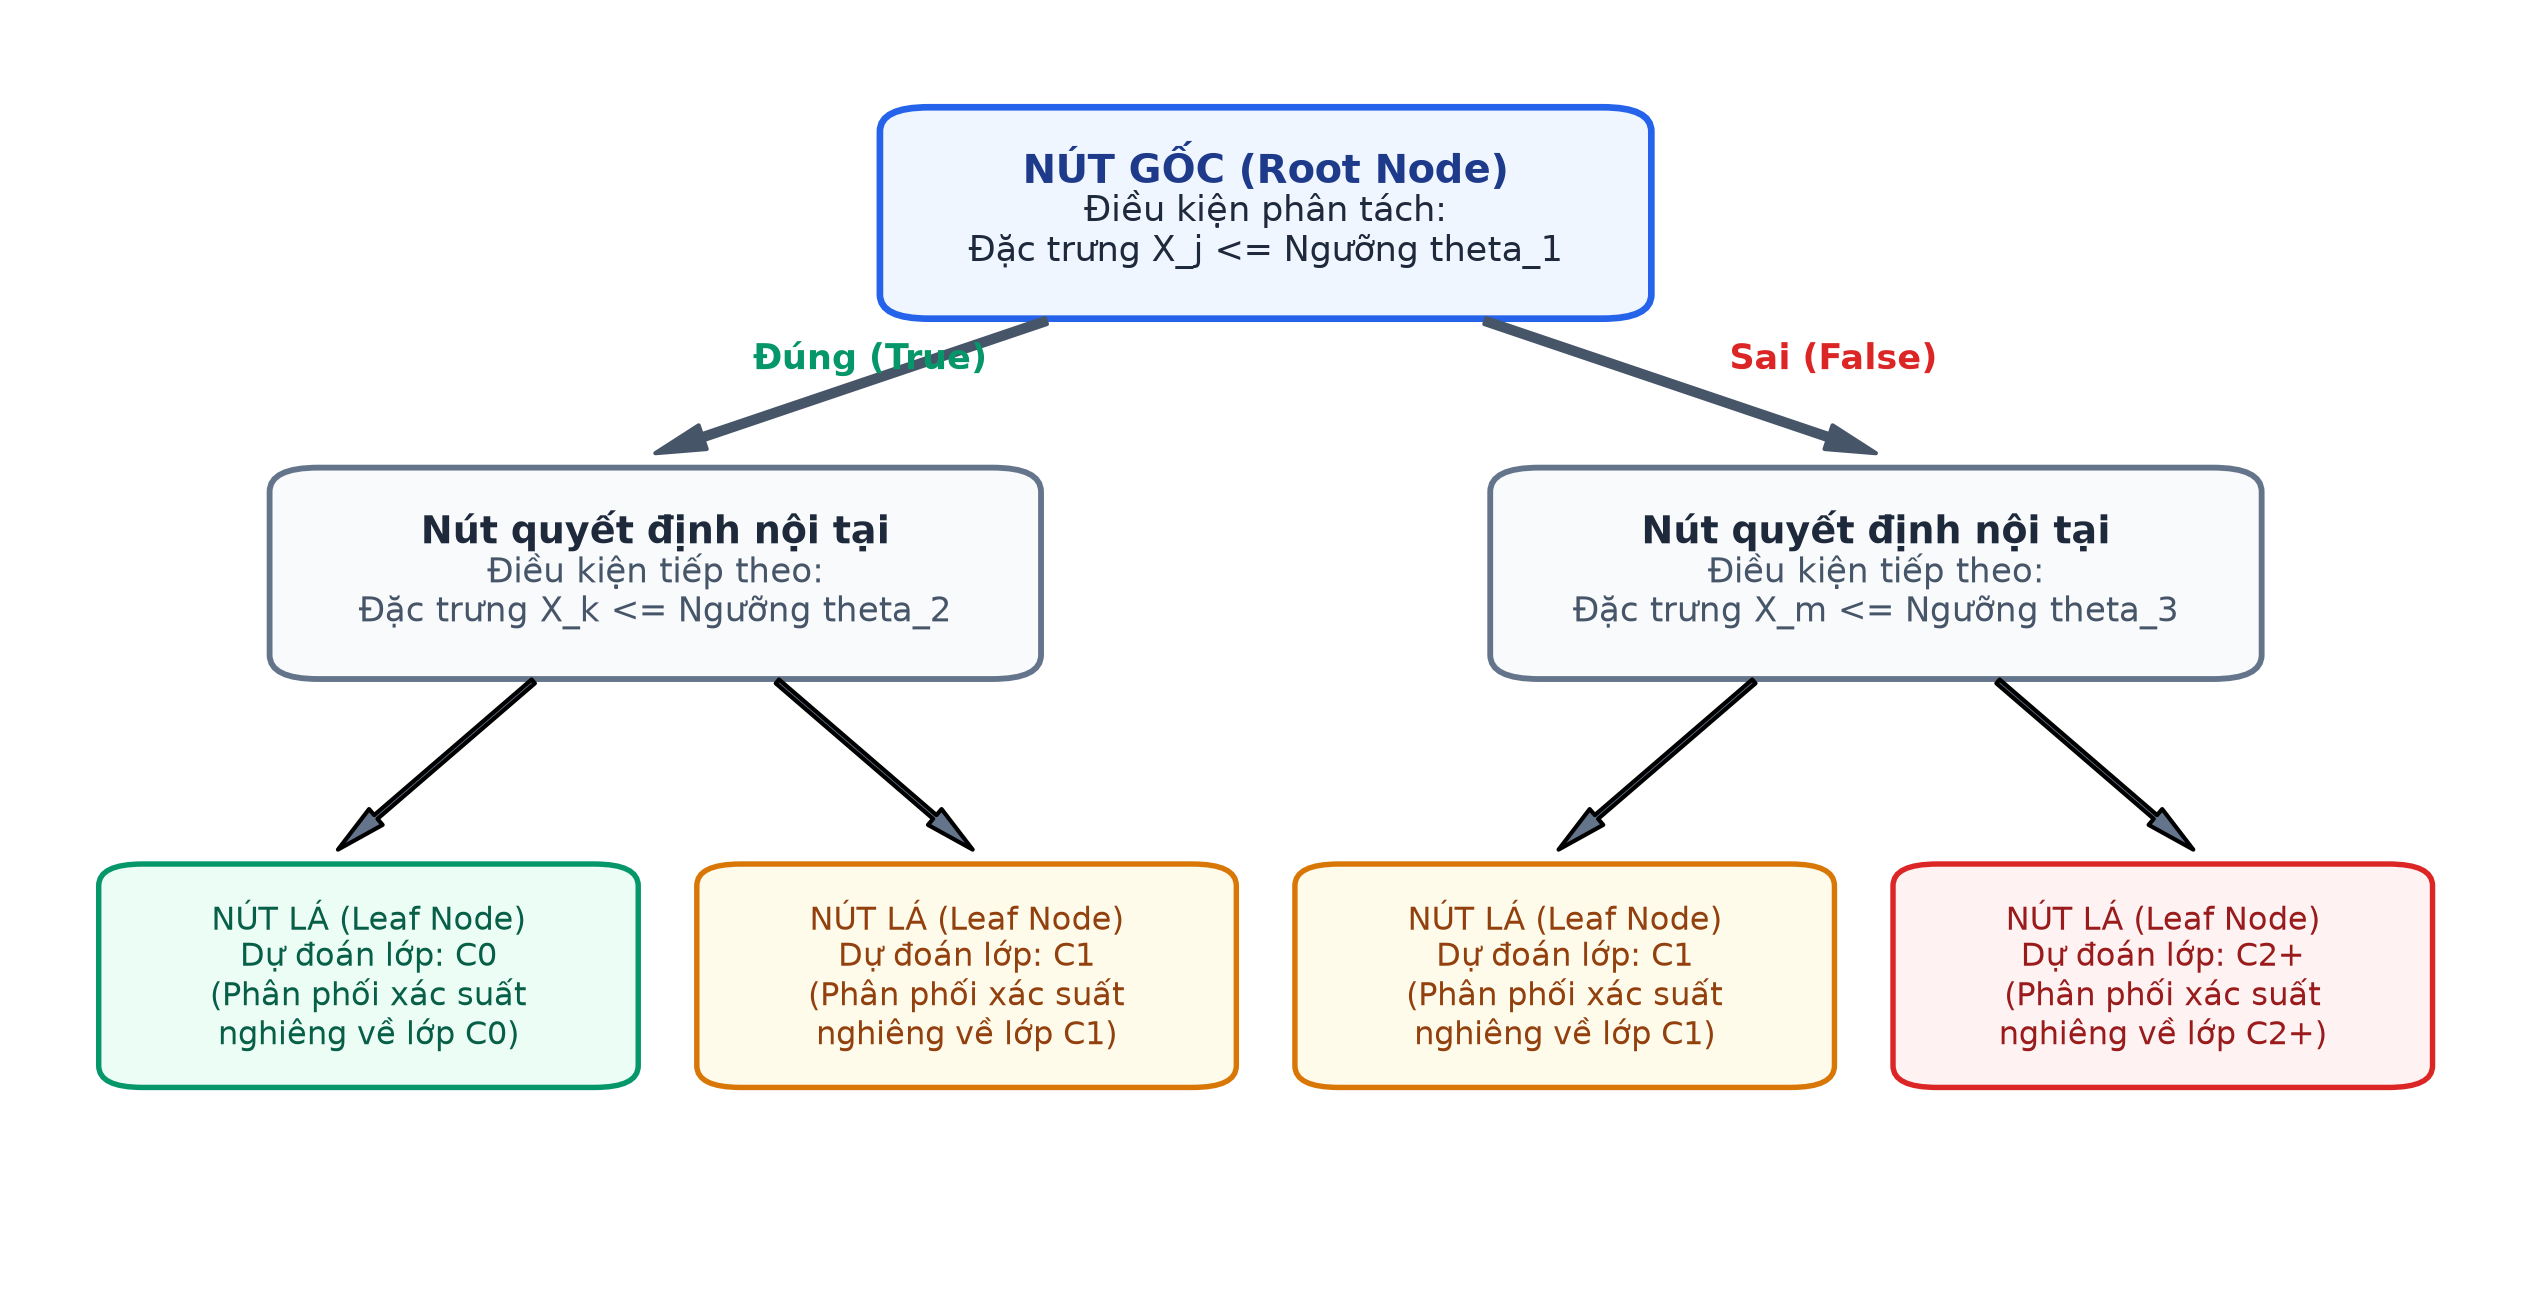
\includegraphics[width=0.88\textwidth]{figures/fig2_decision_tree_concept.png}
\label{fig:dt-concept}
\end{figure}
\FloatBarrier

Quá trình hoạt động của Decision Tree gồm:
\begin{enumerate}
    \item \textbf{Cấu trúc phân cấp:} Cây bắt đầu từ một nút gốc (Root Node) chứa toàn bộ tập dữ liệu huấn luyện, phân nhánh qua các nút quyết định (Decision Nodes) và kết thúc tại các nút lá (Leaf Nodes).
    \item \textbf{Quy tắc phân tách nhị phân:} Tại mỗi nút, thuật toán tìm kiếm đặc trưng $X_j$ và ngưỡng cắt $\theta$ tối ưu để chia dữ liệu thành hai nhánh con: $X_j \le \theta$ và $X_j > \theta$.
    \item \textbf{Tiêu chuẩn độ bất thuần Gini (Gini Impurity):} Cặp $(X_j, \theta)$ được chọn sao cho mức giảm độ bất thuần là lớn nhất. Chỉ số Gini tại một nút được định nghĩa:
    \begin{equation}
        G = 1 - \sum_{k=0}^{K-1} p_k^2
    \end{equation}
    trong đó $p_k$ là tỷ lệ mẫu thuộc lớp $k$ tại nút đó. Khi nút chỉ chứa mẫu của một lớp duy nhất, $G = 0$ (thuần khiết).
    \item \textbf{Dự đoán tại nút lá:} Khi cây đạt tiêu chuẩn dừng (độ sâu tối đa, số lượng mẫu tối thiểu tại lá), nút trở thành nút lá. Xác suất gán cho từng lớp tại lá là tỷ lệ mẫu thực tế của các lớp rơi vào vùng không gian con đó.
\end{enumerate}

\textbf{Hạn chế của Decision Tree đơn lẻ:} Một cây quyết định đơn lẻ có \textbf{phương sai cao (high variance)}. Do cây phân nhánh theo thuật toán tham lam từ trên xuống dưới, chỉ một biến động nhỏ trong dữ liệu huấn luyện (như một vài mẫu nhiễu) cũng có thể làm thay đổi quyết định phân tách ở nút gốc, kéo theo sự thay đổi toàn bộ cấu trúc các tầng bên dưới. Hiện tượng này khiến cây đơn lẻ dễ bị quá khớp (overfitting) trên dữ liệu y tế dạng bảng.

\subsection{Nguyên lý Random Forest và Cơ chế kết hợp nhiều cây}
\label{subsec:random-forest-deepdive}

Random Forest do Leo Breiman đề xuất năm 2001 \cite{breiman2001random} là phương pháp học kết hợp giúp khắc phục nhược điểm phương sai cao của cây đơn lẻ bằng cách xây dựng một tập hợp gồm $B$ cây quyết định độc lập (Hình \ref{fig:rf-concept}).

\begin{figure}[htbp]{Kiến trúc Random Forest: Bootstrap Sampling, ngẫu nhiên hóa đặc trưng và tổng hợp Soft Voting}
\centering
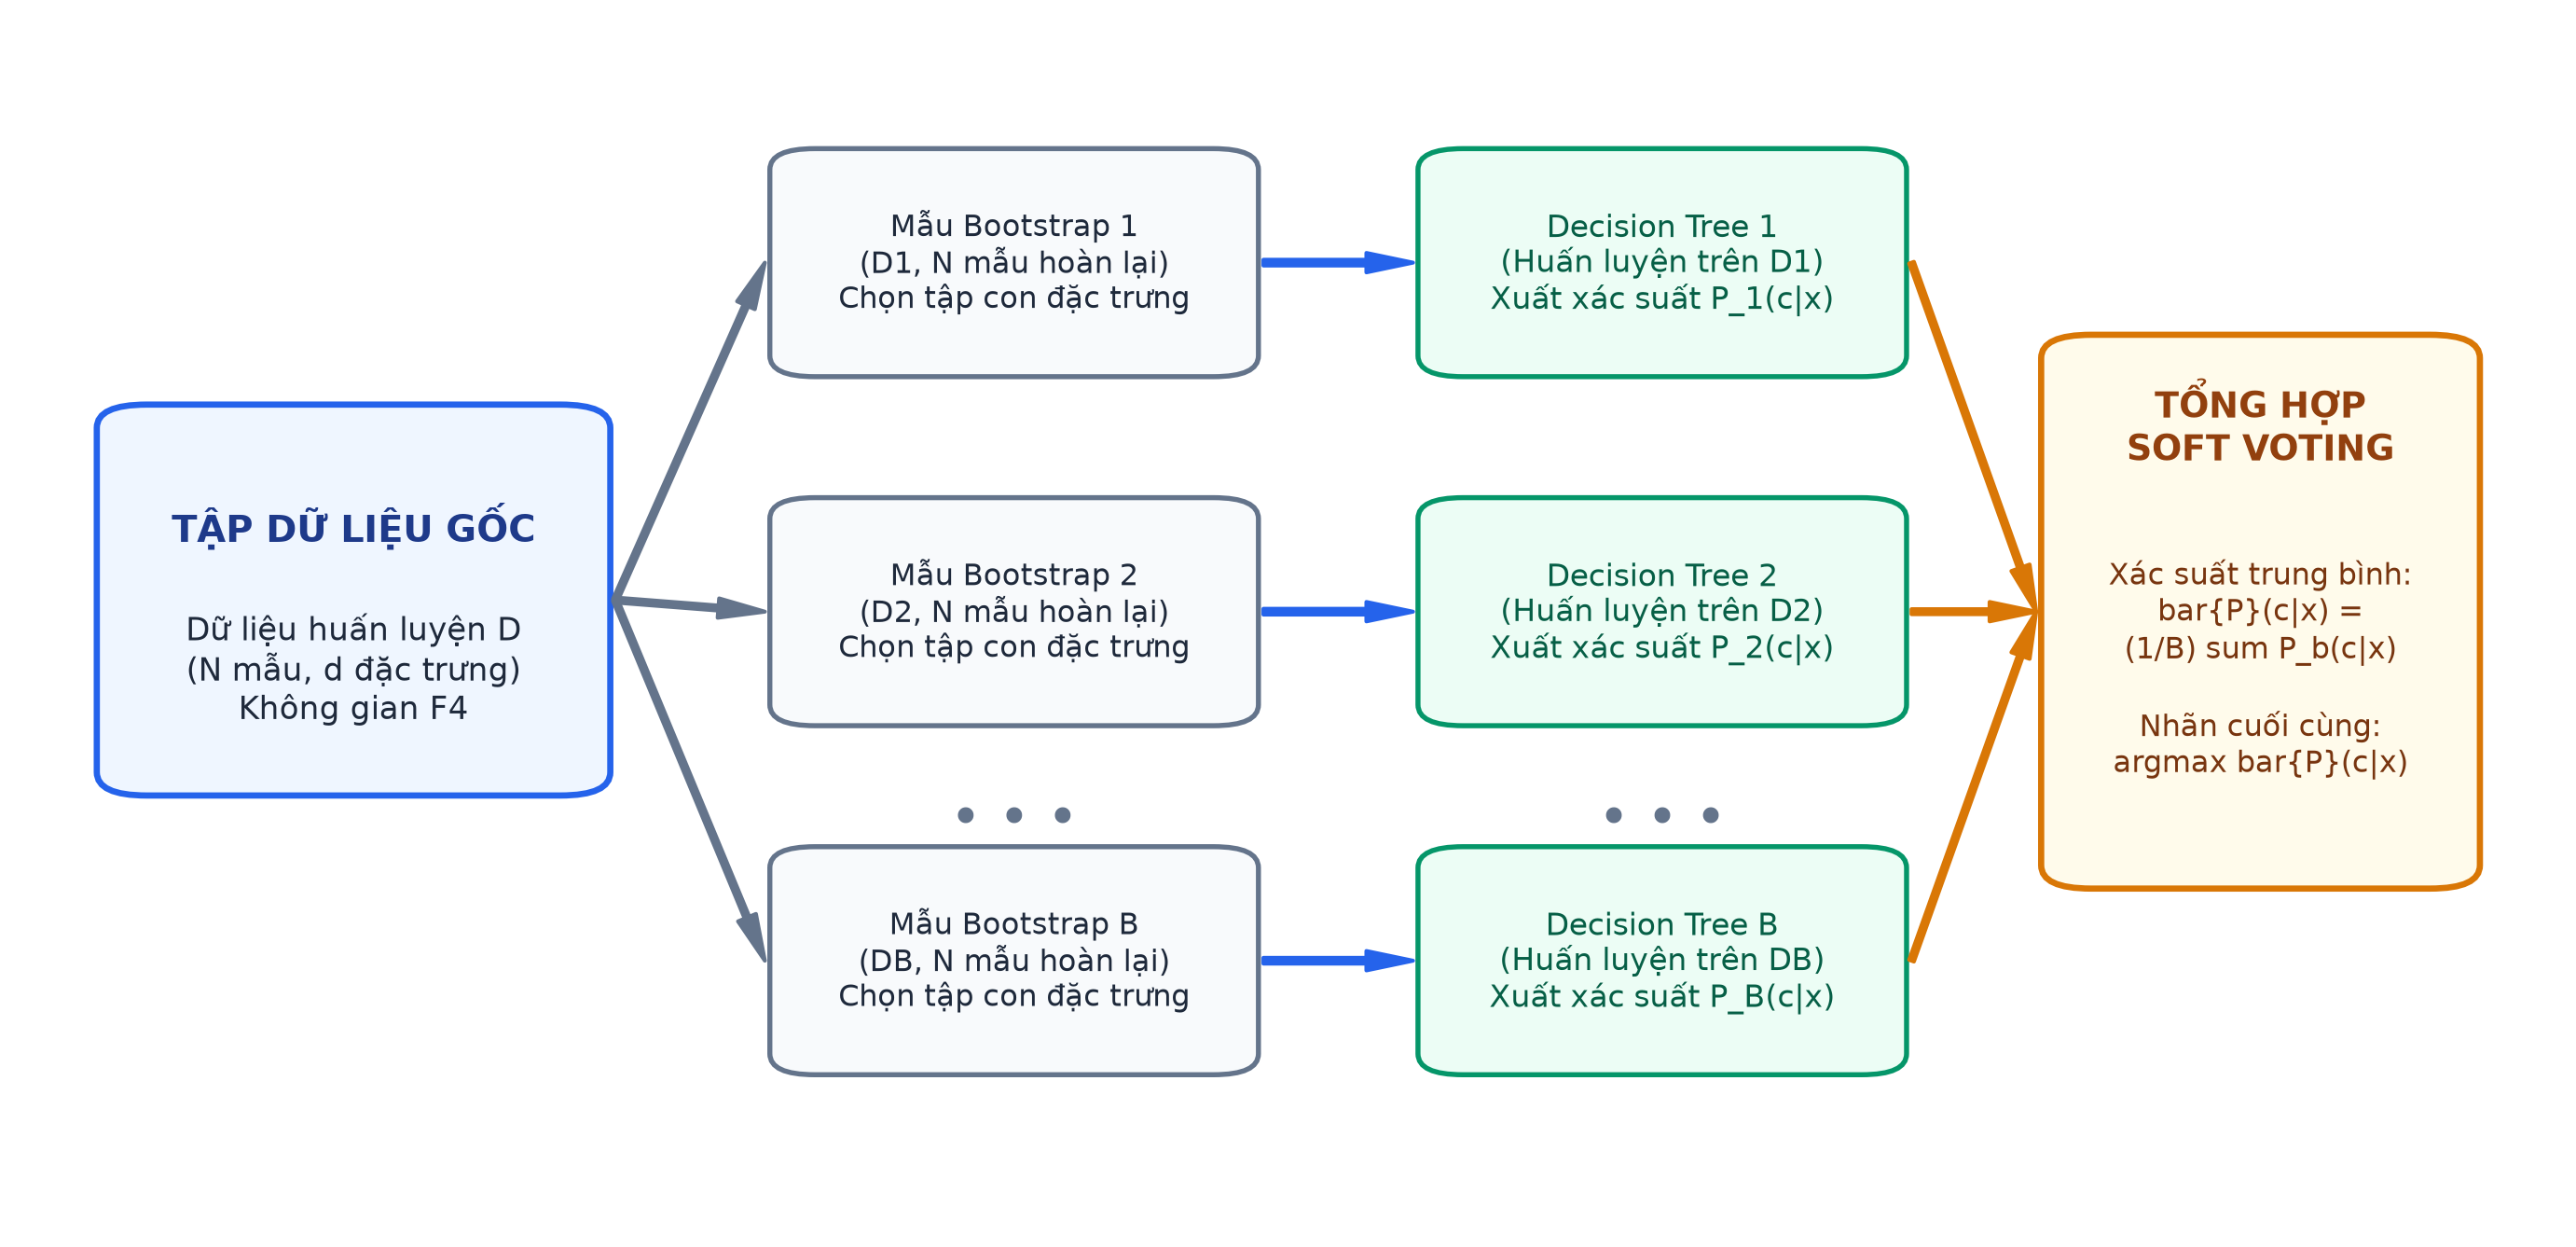
\includegraphics[width=\textwidth]{figures/fig2_random_forest_architecture.png}
\label{fig:rf-concept}
\end{figure}
\FloatBarrier

Random Forest vận hành dựa trên ba cơ chế chính:
\begin{enumerate}
    \item \textbf{Kỹ thuật Bootstrap Sampling:}
    Từ tập dữ liệu huấn luyện gốc gồm $N$ mẫu, thuật toán rút ngẫu nhiên có hoàn lại (sampling with replacement) đúng $N$ lần để tạo ra $B$ tập dữ liệu con độc lập $\mathcal{D}_1, \dots, \mathcal{D}_B$. Mỗi tập con chứa trung bình khoảng 63.2\% số mẫu độc nhất từ tập gốc, phần còn lại (khoảng 36.8\%) không xuất hiện trong tập huấn luyện của cây đó và được gọi là tập ngoài túi (Out-Of-Bag -- OOB).
    \item \textbf{Ngẫu nhiên hóa không gian đặc trưng (Feature Subspace Sampling):}
    Tại mỗi bước phân nhánh của từng cây con, Random Forest chỉ cho phép thuật toán chọn ngẫu nhiên một tập con gồm $m < d$ đặc trưng (trong nghiên cứu này đặt $m = 0.5 \times d$). Thuật toán chỉ tìm kiếm điểm cắt tối ưu trên tập con $m$ đặc trưng này. Nhờ đó, các cây con giảm bớt độ tương quan với nhau và khai thác thông tin từ nhiều góc nhìn khác nhau.
    \item \textbf{Cơ chế giảm phương sai bằng trung bình nhiều cây:}
    Việc lấy trung bình dự đoán từ nhiều cây quyết định được huấn luyện trên các tập mẫu và không gian đặc trưng ngẫu nhiên giúp triệt tiêu phần lớn phương sai ngẫu nhiên của từng cây đơn lẻ mà không làm tăng độ lệch (bias). Kết quả là mô hình tổng hợp đạt được tính ổn định và khả năng khái quát hóa tốt hơn nhiều so với một cây đơn lẻ.
\end{enumerate}

\subsection{Quy trình suy luận của một mẫu dữ liệu qua Random Forest}
\label{subsec:rf-inference-pipeline}

Khi một mẫu dữ liệu mới với vectơ đặc trưng $\mathbf{x} \in \mathbb{R}^d$ được đưa vào Random Forest, quy trình suy luận diễn ra qua các bước:
\begin{enumerate}
    \item Mẫu $\mathbf{x}$ được đưa đồng thời qua $B = 150$ cây quyết định trong rừng.
    \item Tại mỗi cây $b \in \{1, \dots, B\}$, mẫu di chuyển theo các ranh giới rẽ nhánh từ nút gốc xuống nút lá. Tỷ lệ các lớp mẫu tại nút lá tạo thành vectơ phân phối xác suất dự đoán của cây đó:
    \begin{equation}
        \mathbf{p}_b(\mathbf{x}) = \left[ P_b(Y = 0 \mid \mathbf{x}), \, P_b(Y = 1 \mid \mathbf{x}), \, \dots, \, P_b(Y = K-1 \mid \mathbf{x}) \right]^T
    \end{equation}
    \item Toàn bộ mô hình tổng hợp các dự đoán qua cơ chế \textbf{Soft Voting} (lấy trung bình cộng xác suất của tất cả các cây):
    \begin{equation}
        \bar{P}(Y = k \mid \mathbf{x}) = \frac{1}{B} \sum_{b=1}^B P_b(Y = k \mid \mathbf{x})
    \end{equation}
    Khác với Hard Voting (chỉ đếm số phiếu của lớp chiếm đa số), Soft Voting giữ lại độ tự tin định lượng của từng cây con, tạo ra phân phối xác suất trơn mượt phục vụ cho các bước phân cấp và tối ưu rủi ro chi phí tiếp theo.
    \item Trong mô hình phân loại phẳng, nhãn dự đoán cuối cùng là lớp có xác suất trung bình lớn nhất: $\hat{y} = \arg\max_k \bar{P}(Y = k \mid \mathbf{x})$.
\end{enumerate}

\subsection{Vai trò của các siêu tham số Random Forest trong dự án}
\label{subsec:rf-hyperparameters-role}

Trong dự án DepSev-ML, cấu hình Random Forest được cố định dựa trên kết quả tối ưu từ Nested CV:
\begin{itemize}
    \item \texttt{n\_estimators = 150}: Số lượng cây trong rừng. Giá trị $B = 150$ đủ để phân phối xác suất ổn định mà không gây tốn kém thời gian tính toán.
    \item \texttt{max\_depth = 8}: Độ sâu tối đa của từng cây. Giới hạn độ sâu ở mức 8 giúp cây không phân nhánh quá chi tiết để khớp các mẫu nhiễu, hạn chế tình trạng quá khớp.
    \item \texttt{max\_features = 0.5}: Tỷ lệ đặc trưng được chọn tại mỗi nút phân nhánh. Với không gian 34 biến ($F_4$), mỗi nút chỉ xem xét ngẫu nhiên 17 biến, giúp giảm độ tương quan giữa các cây.
    \item \texttt{min\_samples\_split = 10} và \texttt{min\_samples\_leaf = 8}: Số mẫu tối thiểu để phân nhánh và tại nút lá, bảo đảm phân phối xác suất tại nút lá có đủ số lượng mẫu quan sát.
    \item \texttt{class\_weight = 'balanced\_subsample'}: Cơ chế điều chỉnh trọng số nghịch đảo tần số lớp trên từng mẫu bootstrap riêng biệt:
    \begin{equation}
        w_k^{(b)} = \frac{N^{(b)}}{K \cdot N_k^{(b)}}
    \end{equation}
    Kỹ thuật này giúp các cây quyết định chú ý hơn đến các mẫu thuộc lớp thiểu số trong từng lượt lấy mẫu.
\end{itemize}

\section{Các trường phái mô hình hóa trong bài toán phân loại thứ bậc}
\label{sec:truong-phai-mo-hinh-hoa}

Để xử lý bài toán phân tầng mức độ triệu chứng, nghiên cứu khảo sát ba trường phái mô hình hóa chính được minh họa trong Hình \ref{fig:modeling-paradigms}.

\begin{figure}[htbp]{Ba trường phái mô hình hóa: (a) Phân loại phẳng, (b) Phân loại phân cấp hai giai đoạn, và (c) Phân loại thứ bậc}
\centering
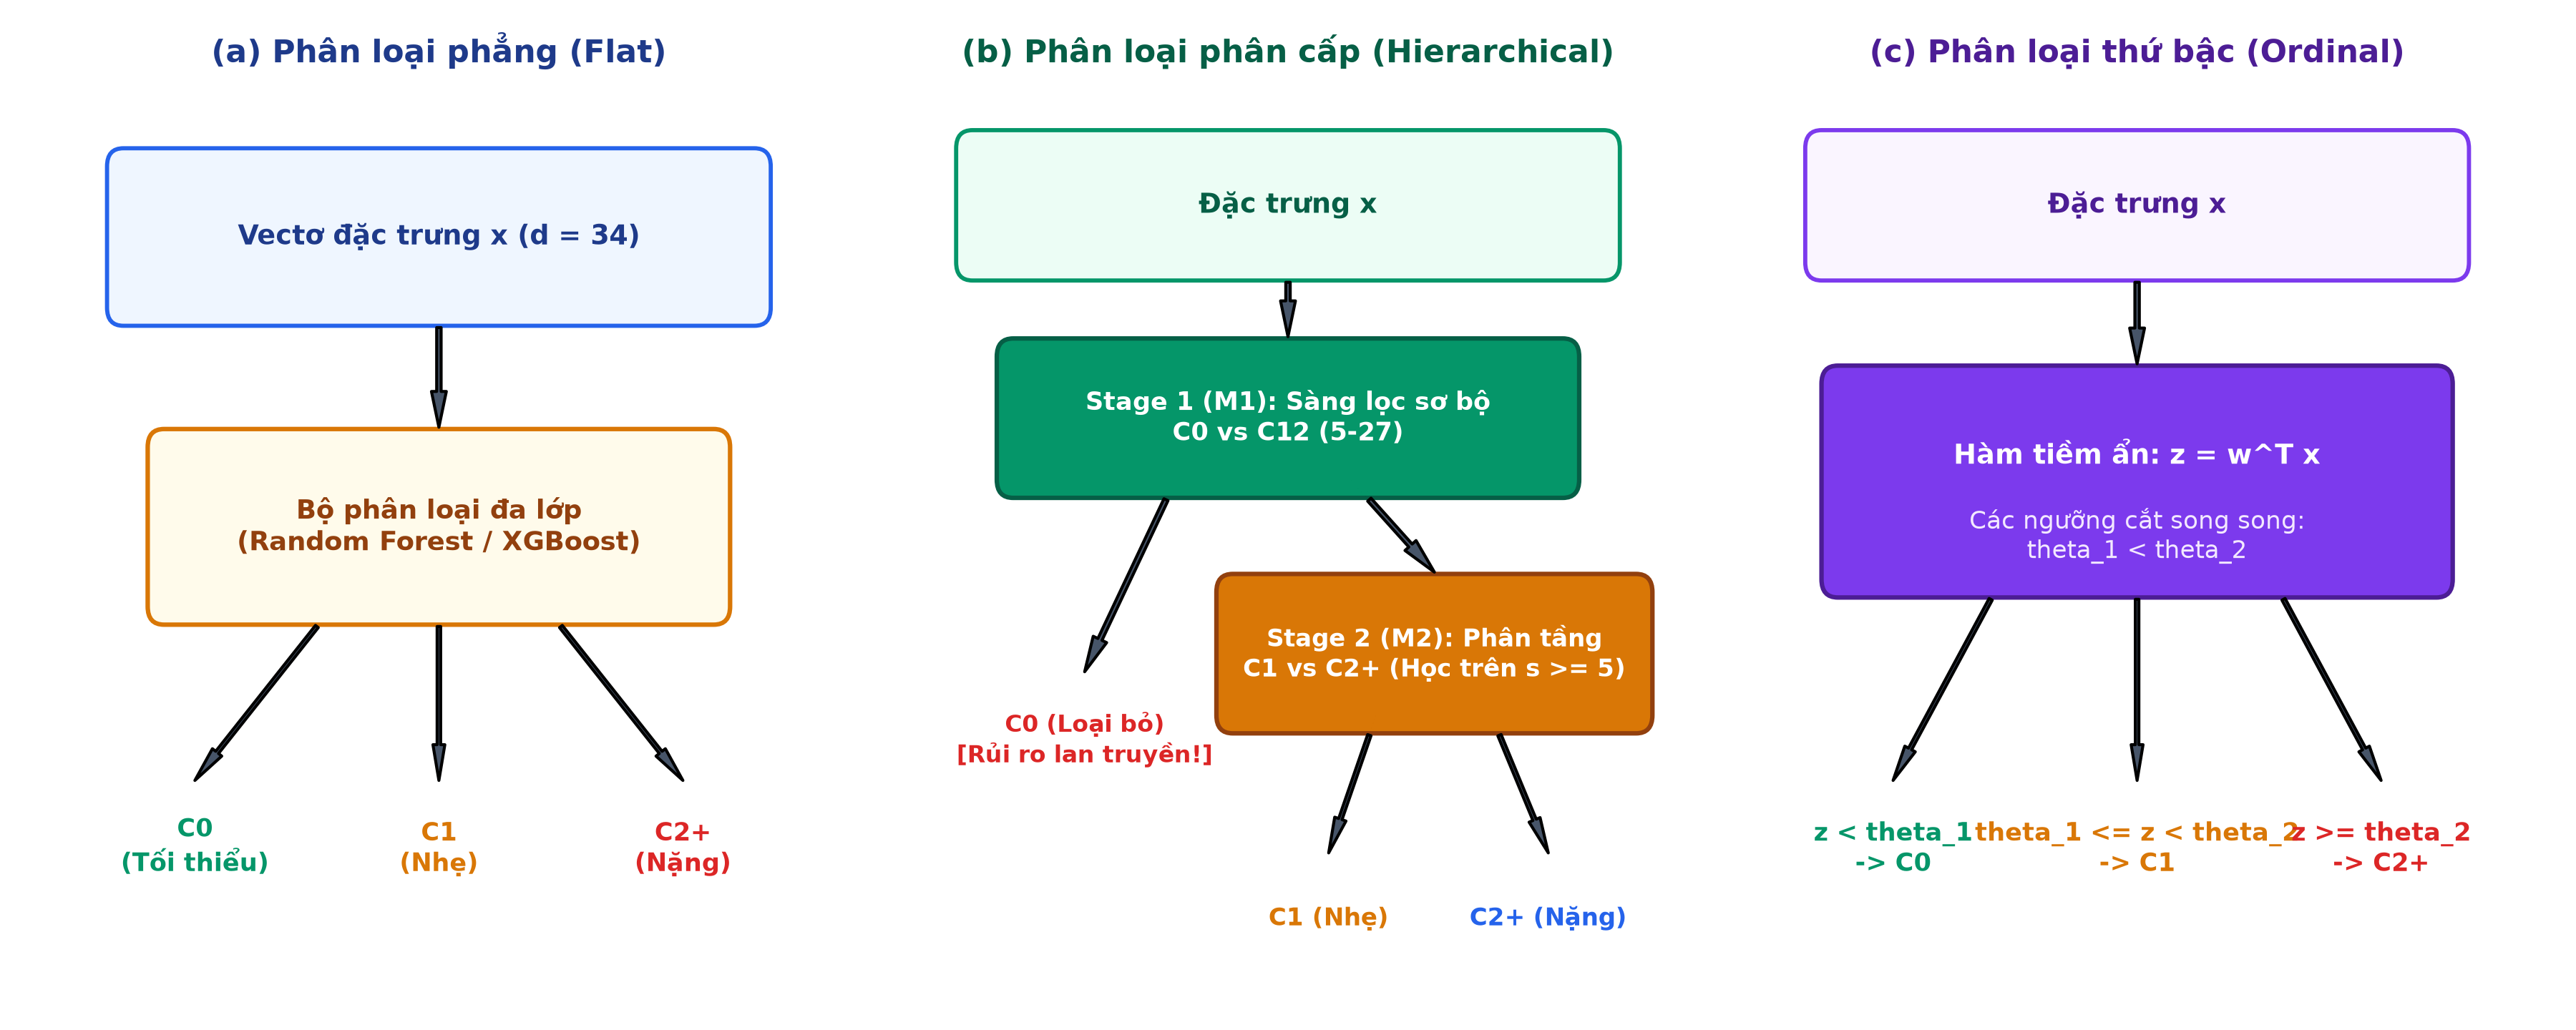
\includegraphics[width=\textwidth]{figures/fig2_modeling_paradigms.png}
\label{fig:modeling-paradigms}
\end{figure}
\FloatBarrier

\subsection{Trường phái phân loại phẳng (Flat Classification)}
\label{subsec:flat-paradigm}

Cách tiếp cận phân loại phẳng coi $K$ mức độ nghiêm trọng là các nhãn danh nghĩa hoàn toàn độc lập. Mô hình học trực tiếp một hàm ánh xạ $f: \mathbb{R}^d \to \Delta^K$ để dự đoán phân phối xác suất hậu nghiệm $P(Y = k \mid \mathbf{x})$. Các thuật toán cơ sở gồm Logistic Regression, Random Forest và XGBoost.

Hạn chế của trường phái phẳng là bỏ qua quan hệ thứ tự tự nhiên giữa các mức độ ($C_0 < C_1 < C_2$). Sai số nhầm lẫn giữa $C_0$ và $C_1$ (chênh 1 bậc) bị hàm mất mát đánh giá ngang bằng với sai số giữa $C_0$ và $C_2^+$ (chênh 2 bậc). Đồng thời, khi dữ liệu mất cân bằng lớn, ranh giới phân tách phẳng dễ bị đẩy ép về phía lớp thiểu số.

\subsection{Trường phái phân loại phân cấp (Hierarchical Classification)}
\label{subsec:hierarchical-paradigm}

Nhằm mô phỏng quy trình sàng lọc hai bước (trước hết nhận diện người có triệu chứng, sau đó mới phân tầng mức độ), trường phái phân cấp chia nhỏ bài toán thành cấu trúc gồm hai giai đoạn \cite{silla2011survey}:
\begin{itemize}
    \item \textbf{Giai đoạn 1 (Bộ phân loại sàng lọc $M_1$):} Phân loại nhị phân giữa nhóm triệu chứng tối thiểu ($C_0$) và nhóm có triệu chứng ($C_{12} = C_1 \cup C_2^+$).
    \item \textbf{Giai đoạn 2 (Bộ phân loại phân tầng $M_2$):} Trong số các mẫu có triệu chứng, phân biệt giữa mức độ nhẹ ($C_1$) và mức độ nặng theo quy ước ($C_2^+$).
\end{itemize}

Kiến trúc phân cấp được thử nghiệm với hai cơ chế định tuyến:
\begin{enumerate}
    \item \textbf{Định tuyến cứng (Hard Routing):} Nếu $M_1$ dự đoán một mẫu là $C_0$, mẫu đó lập tức được gán nhãn $C_0$ và kết thúc luồng. Cơ chế này dẫn đến hiện tượng \textbf{lan truyền sai số một chiều (Error Propagation)}: nếu một mẫu nặng $C_2^+$ bị $M_1$ gán nhầm thành $C_0$, sai sót này không thể sửa chữa ở Giai đoạn 2.
    \item \textbf{Định tuyến mềm (Soft Routing):} Cả hai mô hình $M_1$ và $M_2$ đều xuất ra xác suất liên tục. Xác suất kết hợp toàn phần được tính bởi:
    \begin{align}
        \hat{P}(C_0 \mid \mathbf{x}) &= P_{M_1}(C_0 \mid \mathbf{x}) \\
        \hat{P}(C_1 \mid \mathbf{x}) &= P_{M_1}(C_{12} \mid \mathbf{x}) \cdot P_{M_2}(C_1 \mid C_{12}, \mathbf{x}) \\
        \hat{P}(C_2^+ \mid \mathbf{x}) &= P_{M_1}(C_{12} \mid \mathbf{x}) \cdot P_{M_2}(C_2^+ \mid C_{12}, \mathbf{x})
    \end{align}
    Cơ chế mềm bảo toàn thông tin xác suất liên tục và cho phép các bước sau linh hoạt điều chỉnh ngưỡng quyết định.
\end{enumerate}

\subsection{Lý thuyết quyết định nhạy chi phí Bayes (Bayes Cost-Sensitive Decision)}
\label{subsec:cost-sensitive-paradigm}

Trong sàng lọc y tế, các loại sai lầm có mức độ ảnh hưởng khác nhau: việc bỏ sót một ca bệnh nặng ($C_2^+ \to C_0$) thường mang lại rủi ro lớn hơn so với một ca báo động nhầm ($C_0 \to C_2^+$). Lý thuyết quyết định nhạy chi phí Bayes \cite{elkan2001foundations} cung cấp cơ sở toán học để tối ưu quyết định dưới sự bất cân xứng này.

Quy ước ma trận chi phí $\mathbf{C} \in \mathbb{R}^{K \times K}$, trong đó phần tử $\mathbf{C}(i, j)$ là chi phí phạt khi nhãn thực tế là $i$ và nhãn dự đoán là $j$ (với $\mathbf{C}(i, i) = 0$). Rủi ro kỳ vọng của việc dự đoán lớp $j$ với mẫu có vectơ xác suất $\hat{\mathbf{P}}$ là:
\begin{equation}
    R(j \mid \mathbf{x}) = \sum_{i=0}^{K-1} \hat{P}(C_i \mid \mathbf{x}) \cdot \mathbf{C}(i, j)
\end{equation}
Quy tắc quyết định tối ưu Bayes là chọn nhãn $\hat{y}^*$ có rủi ro kỳ vọng nhỏ nhất:
\begin{equation}
    \hat{y}^* = \arg\min_{j \in \{0, \dots, K-1\}} R(j \mid \mathbf{x})
\end{equation}
Bằng cách gán trọng số phạt lớn cho phần tử $\mathbf{C}(2, 0)$ (nhãn thật là $C_2^+$, dự đoán nhầm thành $C_0$), mô hình chủ động dịch chuyển ranh giới quyết định để giảm thiểu số ca nặng bị bỏ sót, chấp nhận một mức độ gia tăng hợp lý của các ca báo động nhầm.

\subsection{Trường phái phân loại thứ bậc (Ordinal Classification)}
\label{subsec:ordinal-paradigm}

Do các mức độ triệu chứng PHQ-9 có tính chất thứ bậc ($C_0 < C_1 < C_2$), phân loại thứ bậc khai thác cấu trúc trật tự này để hạn chế các sai số nhảy bậc lớn \cite{mccullagh1980regression, frank2001simple}:
\begin{enumerate}
    \item \textbf{Mô hình Ordinal Logistic Regression (OLR):} Giả định tồn tại một biến tiềm ẩn tuyến tính $z = \mathbf{w}^T \mathbf{x}$ và tập hợp các ngưỡng cắt đơn điệu $\theta_1 < \theta_2 < \dots < \theta_{K-1}$. Xác suất tích lũy được mô hình hóa theo hàm phân phối Logistic:
    \begin{equation}
        P(Y \le k \mid \mathbf{x}) = \sigma(\theta_{k+1} - \mathbf{w}^T \mathbf{x}) = \frac{1}{1 + e^{-(\theta_{k+1} - \mathbf{w}^T \mathbf{x})}}
    \end{equation}
    Mô hình OLR sử dụng chung một vectơ trọng số $\mathbf{w}$ cho tất cả các ranh giới (giả định proportional odds), giúp số lượng tham số gọn và các siêu phẳng quyết định song song không bao giờ cắt nhau.
    \item \textbf{Phân loại nhị phân tích lũy (Cumulative Binary Classification -- CBC):} Huấn luyện $K-1$ bộ phân loại nhị phân độc lập $h_k(\mathbf{x})$ để dự đoán biến cố tích lũy $P(Y \ge k \mid \mathbf{x})$. Tuy nhiên, phương pháp này tiềm ẩn nguy cơ vi phạm tính đơn điệu xác suất khi xuất hiện $P(Y \ge k+1) > P(Y \ge k)$ trên một số mẫu dữ liệu ngoài mẫu.
\end{enumerate}

\section{Tổng quan các nghiên cứu liên quan}
\label{sec:nghien-cuu-lien-quan}

Trong những năm gần đây, việc áp dụng học máy trên dữ liệu khảo sát NHANES để nghiên cứu trầm cảm đã được quan tâm trong y văn. Bảng \ref{tab:related-works} tổng hợp các công trình tiêu biểu liên quan.

\begin{table}{Tổng hợp so sánh các nghiên cứu liên quan về dự đoán trầm cảm từ dữ liệu y tế}
\centering
\footnotesize
\setlength{\tabcolsep}{3pt}
\label{tab:related-works}
\begin{tabularx}{\textwidth}{p{3.2cm} p{2.2cm} p{2.4cm} p{2.8cm} X}
\toprule
\textbf{Nghiên cứu} & \textbf{Nguồn dữ liệu} & \textbf{Không gian đích} & \textbf{Phương pháp học máy} & \textbf{Đặc điểm và Hạn chế} \\
\midrule
Pratt và cộng sự (2014) \cite{pratt2014depression} & NHANES 2009--2012 & Nhị phân ($s \ge 10$) & Thống kê dịch tễ mô tả, Hồi quy đa biến & Tập trung phân tích tương quan dịch tễ, không xây dựng mô hình dự đoán Machine Learning. \\
\midrule
Patel và cộng sự (2016) \cite{patel2016systematic} & NHANES đa chu kỳ & Nhị phân ($s \ge 10$) & Logistic Regression, Decision Tree & Chỉ khảo sát bài toán nhị phân, chưa phân tầng đa mức độ triệu chứng. \\
\midrule
Dipnall và cộng sự (2016) \cite{dipnall2016fusing} & Dữ liệu lâm sàng & Nhị phân ($s \ge 10$) & Phân tích chỉ dấu sinh học, PCA, GLM & Đánh giá trên tập mẫu hạn chế, chưa kiểm tra rò rỉ dữ liệu qua Nested CV. \\
\midrule
Zhang và cộng sự (2020) \cite{zhang2020machine} & Khảo sát cộng đồng & Đa lớp (3 mức) & Random Forest, XGBoost phẳng & Áp dụng mô hình phẳng, chưa tối ưu chi phí cho các ca nặng. \\
\midrule
Kaggle Benchmark CDC (2021) & NHANES 2013--2014 & Nhị phân / 5 lớp & Baseline Ensembles, Deep ANN & Đánh giá chủ yếu qua Accuracy, không phân tích đánh đổi sai số lâm sàng. \\
\midrule
\textbf{DepSev-ML (Nghiên cứu này)} & \textbf{NHANES 3 chu kỳ (2011--2016)} & \textbf{Đa mức ($T_2, T_3, T_4, T_5$)} & \textbf{Phân cấp mềm, Quyết định Bayes, Ordinal} & \textbf{Khảo sát quy luật suy thoái theo độ chi tiết, tối ưu chi phí bỏ sót ca nặng và kiểm định ngoại suy theo thời gian.} \\
\bottomrule
\end{tabularx}
\end{table}

Qua khảo sát y văn, có thể rút ra một số khoảng trống nghiên cứu chính:
\begin{enumerate}
    \item Đa số các công trình trước đây tập trung vào bài toán nhị phân thô ($s \ge 10$ hoặc $s \ge 5$). Rất ít nghiên cứu khảo sát sự suy giảm hiệu năng khi mở rộng sang bài toán đa mức ($T_3 \to T_5$).
    \item Các nghiên cứu đa mức hiện có chủ yếu sử dụng mô hình phẳng truyền thống, chưa khai thác cấu trúc thứ bậc và chưa lượng hóa sự đánh đổi giữa việc giảm bỏ sót ca nặng và gia tăng báo động nhầm.
    \item Chưa có nhiều công trình đánh giá có đối chứng giữa phân cấp cứng và phân cấp mềm kết hợp tối ưu chi phí Bayes, cũng như kiểm tra tính ổn định của mô hình trên tập dữ liệu tương lai độc lập.
\end{enumerate}

\section{Tóm tắt chương}
\label{sec:tom-tat-chuong-2}

Chương 2 đã trình bày cơ sở lý thuyết về thang đo PHQ-9, các cơ chế sinh học liên quan đến triệu chứng trầm cảm, và hai thách thức chính của dữ liệu dạng bảng là mất cân bằng lớp và chồng lấn đặc trưng. Chương cũng đã phân tích chi tiết nguyên lý hoạt động của Random Forest và ba trường phái mô hình hóa (phẳng, phân cấp, thứ bậc). Các nội dung này là cơ sở trực tiếp để xây dựng phương pháp và quy trình thực nghiệm trong Chương \ref{ch:phuong-phap}.
